\chapter{Analyse de l'existant}

Dans le cadre du projet, nous avons besoin : 

\begin{itemize}
    \item D'un serveur de route permettant de diffuser auprès des routeurs les mises à jour des routes.
    \item D'un framework pour le Frontend
    \item D'un framework pour le Backend
    \item D'un outil de virtualisation pour réaliser les tests d'acceptation.
\end{itemize}

\section{ExaBGP}
\textbf{Version ExaBGP 3.4.26}

ExaBGP \cite{Exa13} est une application conçue pour permettre aux programmeurs et aux administrateurs réseaux d’interagir facilement avec les réseaux BGP. Il fut développé en 2010. Le programme est conçu pour permettre l’injection de routes dans un réseau, y compris IPv6 et FlowSpec \cite{Man10}.

Cet outil utilise le format JSON pour rendre les messages BGP plus agréables à manipuler. C'est pourquoi, nous devons définir les formats JSON que nous utilisons. Voir la section \hyperref[sssec:exabgp]{Communication avec ExaBGP}.

Nous avons fait le choix d'utiliser une version ultérieure à celle qui fait référence en ce moment. Cela s'explique par le fait que lors de la mise en place de cet outil, nous nous sommes heurté à quelques complications. Malheureusement, cette version utilise \textit{python 2} alors que tous le reste du projet est en \textit{python 3}.

\section{Django}
\textbf{Version Django 2.1.5}

Django \cite{Django03} est un framework utilisant le langage Python. Il a été développé pour facilité le travail des journaliste dans la ville de Lawrence dans le Kansas à partir de 2003 et s'est ouvert au public en 2005. Il est gratuit et open source, consacré au développement Web. Il propose des bases simples et déjà implémentées par d'autres développeurs, comme une page pour l'authentification des utilisateurs ou de quoi gérer le site. Cela permet de grandement faciliter la tâche pour créer une interface Web. 

Nous l'utiliserons en tant que Frontend pour générer une interface utilisateur simple avec authentification. Elle permettra à l'administrateur de gérer les routes. Ces commandes seront ensuite traitées par le Backend. Par conséquent, nous devons définir une \hyperref[sssec:ui]{interface utilisateur}. Ce choix nous est paru judicieux car l'apprentissage de l'utilisation de Django a été rapide et qu'il permet d'avoir une architecture simple et compréhensive rapidement.

\section{Flask-RESTful}
\textbf{Version Flask-RESTful 0.3.7}

\href{https://flask-restful.readthedocs.io/en/latest/}{Flask-RESTful} est une extension du framework Flask permettant de construire des APIs RESTful. Flask a été développé en 2010. Il utilise également le langage Python et permet notamment de faire des sites Web dynamiques, c'est à dire que l'utilisateur pourra interagir avec le site. Cependant, ce qui nous intéresse ici, c'est son module Flask-Restful, l'interface utilisateur étant faite avec Django. Les différentes requêtes HTTP ont leur fonctionnalités codées en Python et peuvent être lancées avec une ligne de commande simple.

Il nous permet de générer une API et de la gérer sans passer l'interface utilisateur, ainsi que d'envoyer des commandes à ExaBGP. Ce module nous permettra de coder les requêtes HTTP et ainsi de pouvoir les exécuter. Nous avons fait le choix de fonctionner en micro service car Django s'intègre difficilement avec MongoDB au contraire de Flask. C'est pourquoi, l'utilisation de Flask nous a paru judicieuse.

\section{MongoDB}
\href{https://www.mongodb.com/fr}{MongoDB} est un système de gestion de base de données orienté sur les documents. MongoDB est développé depuis 2007 par MongoDB. MongoDB permet de manipuler des objets structurés au format BSON (JSON binaire), sans schéma prédéterminé. En d'autres termes, des clés peuvent être ajoutées à tout moment "à la volée", sans reconfiguration de la base. Les données prennent la forme de documents enregistrés eux-mêmes dans des collections, une collection contenant un nombre quelconque de documents. L'avantage de cette base de donnée réside dans sa flexibilité. En effet, chaque champs d'un enregistrement est libre et peuvent être différent d'un enregistrement à un autre au sein d'une même collection. Le seul champs commun obligatoire est le champs d'identifiant, \verb+_i+.

Nous avons fait le choix de stocker nos données sur un serveur distant \href{https://mlab.com/}{mLab} qui nous offre gratuitement l'utilisation d'un serveur MongoDB. Cela nous a permis de travailler sur nos machines sans être dépendant d'un serveur local en supplémentaire. Bien sûr si nous avions des données plus lourdes, il serait plus judicieux d'avoir un serveur local mais ce service nous supporte très bien de multiple requêtes. De plus, cette entreprise a l'avantage de posséder plusieurs serveurs donc le service n'est que très rarement interrompu.

\section{Méthode de virtualisation avec NEmu}
\href{https://gitlab.com/v-a/nemu}{NEmu} (Network Emulator for Mobile Universes) est un environnement de réseaux virtuels distribués, écrit en Python. Il est destiné à l'enseignement et a été élaboré par une équipe de l'Université de Bordeaux. Il gère des machines virtuelles de type QEmu pour construire différentes topologies virtuelles. Ainsi, il possible de relier plusieurs machines entre elles, de simuler des switchs ou des routeurs. Il est également possible, de connecter deux réseaux virtuels différents sur deux machines physiques différentes, correspondant à deux sessions distinctes. On peut également créer plusieurs environnements virtuels, sans qu'ils ne connaissent l'existence les uns des autres.

Ainsi nous pouvons facilement créer un, voire plusieurs ensembles de machine pour figurer un réseau et simuler l'envoie de paquet d'une machine attaquante. Cet outil est fondamental pour les tests d'acceptation que nous mettrons en place. En effet, afin de vérifier que les actions de l'utilisateur ont une répercussion sur le réseau, il faut que l'on crée un environnement avec un attaquant, un client et un serveur de route, une cible ainsi que deux routeurs de frontières.

\section{Erco}
\textit{Apache License Version 2.0, January 2004}

Erco (\textbf{E}xabgp \textbf{R}outes \textbf{CO}ntroller) est un logiciel permettant de piloter ExaBGP \cite{Did15}. Il a été développé par l'Université de Lorraine afin de travailler en relation avec un service de trou noir en temps réel redirigeant le trafic entre un utilisateur et un fournisseur de services Web. C'est un logiciel libre exposant une API REST, lui permettant ainsi d'être utilisé par des programmes.

Il permet l'ajout et la suppression de routes. Voici ce que nous propose la démo du logiciel \cite{Erc16} :

\begin{figure}[H]
\caption{Démo de Erco : Annoncer un nouveau réseau}
\fbox{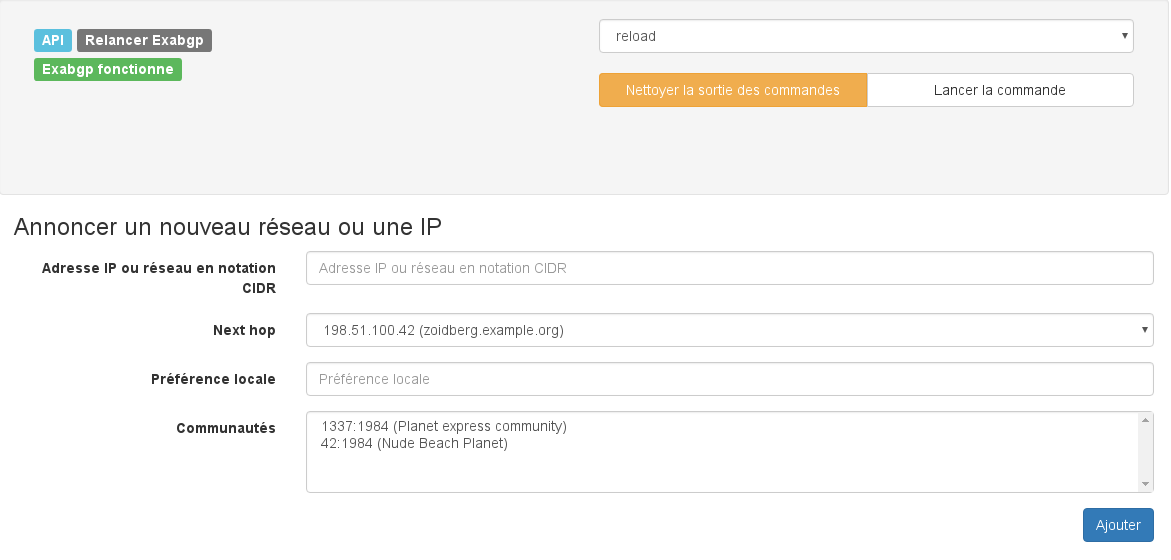
\includegraphics[width=\textwidth]{erco_demo_announce.png}}
\label{fig:erco_demo_announce}
\end{figure}

Sur la figure \ref{fig:erco_demo_announce}, nous pouvons voir que l'on peut facilement lancer une commande, au choix entre : reload, restart, show neighbors, show routes et version. Mais aussi ajouter un nouveau réseau ou une simple machine.

\begin{figure}[H]
\caption{Démo de Erco : Sous-réseaux annoncés}
\fbox{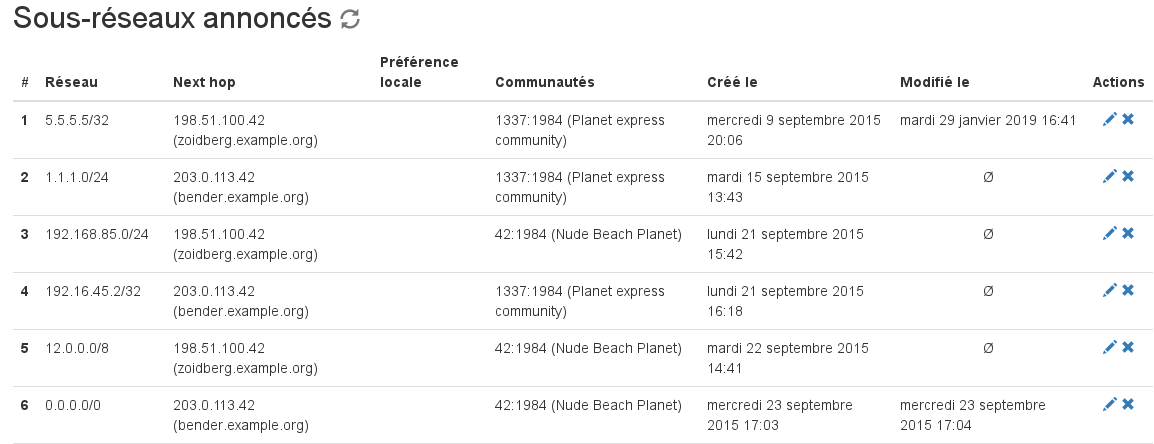
\includegraphics[width=\textwidth]{erco_demo_announced.png}}
\label{fig:erco_announced}
\end{figure}

Sur la figure \ref{fig:erco_announced}, nous pouvons voir la liste des sous-réseaux. Nous pouvons effectuer des actions comme supprimer ou modifier un réseau.

Bien que cette API soit bien constituer, nous ne pouvons pas la reprendre car le client désire que l'on fasse la même API mais avec un langage plus adéquat. En effet, Erco a été programmé en Perl, langage difficilement maintenable par des personnes non expérimentés avec ce langage. Néanmoins, nous allons reprendre tous les formats JSON proposés par l'API ainsi que le même principes des URIs.

\section{Projet de l'an dernier}
Ce projet aura été à la fois simple et difficile à comprendre.

Dans un premier temps, il se sont basés sur le logiciel Erco qui fait quasiment la même chose.

Ils ont également utilisé Meteor, un framework open source de développement Web en JavaScript.
Il leur a permis de développer une API restful permettant l'envoi des commandes pour ajouter ou supprimer des routes. Ils auront dans un premier temps tester sur la console d'une machine si ça s'exécutait bien avant de le faire avec l'API. La figure \ref{fig:meteor_route} montre leur interface utilisateur sous Meteor.

\begin{figure}[H]
\caption{Interface Utilisateur du Projet de l'an dernier}
\fbox{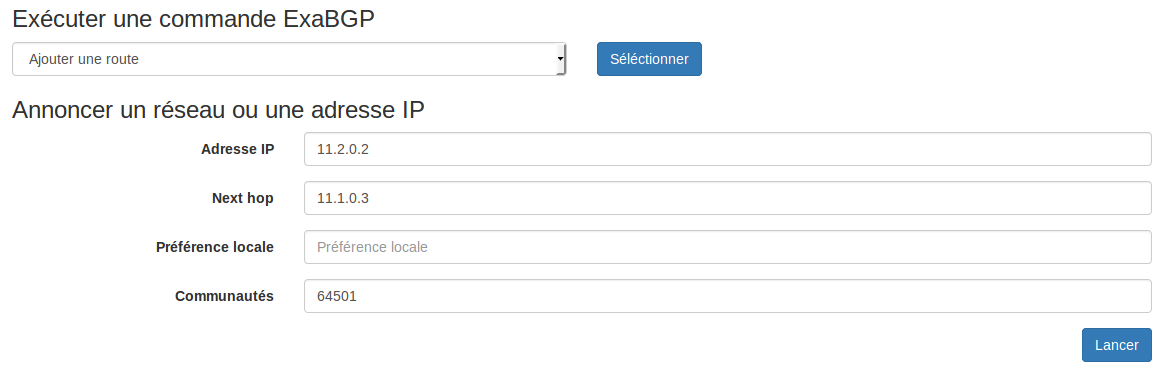
\includegraphics[width=\textwidth]{ajoutRouteMeteor.png}}
\label{fig:meteor_route}
\end{figure}

Pour stocker les modifications concernant les routes, ils ont utilisé une base de données avec MongoDB. C'est également un logiciel open source. 

GNS3 et Nemu leur auront permis de créer un environnement virtuel pour tester leur implémentation. Un read.me est disponible pour configurer l'environnement, pour pouvoir nous même lancer les tests avec leurs travaux. Des installations au préalable doivent être effectuées.
Pour la modification directement sur les routeurs, ils ont utilisés ExaBGP. Recevant les réponses en JSON, ils ont implémenté un convertisseur en python pour les transformer en chaîne de caractère et ainsi pouvoir les envoyer sur les routeurs.

Nous avons décidé de ne pas reprendre le projet de l'an dernier. En effet, nous préférons partir du début car nous n'avons pas les mêmes acquis. De plus, nous serons plus valorisés à recommencer l'implémentation depuis le début, cela mettrait en avant nos compétences. Cependant, nous aurions pu reprendre la partie virtualisation d'un environnement avec différentes machines. Mais, le client nous fourni après la première \textit{releases} les éléments pour aller plus rapidement donc leur travail nous as seulement permis de nous guider sur certaines piste.
